\documentclass[12pt, titlepage]{article}

\usepackage{fullpage}
\usepackage[round]{natbib}
\usepackage{multirow}
\usepackage{booktabs}
\usepackage{tabularx}
\usepackage{graphicx}
\usepackage{float}
\usepackage{hyperref}
\hypersetup{
    colorlinks,
    citecolor=blue,
    filecolor=black,
    linkcolor=red,
    urlcolor=blue
}

%% Comments

\usepackage{color}

\newif\ifcomments\commentstrue %displays comments
%\newif\ifcomments\commentsfalse %so that comments do not display

\ifcomments
\newcommand{\authornote}[3]{\textcolor{#1}{[#3 ---#2]}}
\newcommand{\todo}[1]{\textcolor{red}{[TODO: #1]}}
\else
\newcommand{\authornote}[3]{}
\newcommand{\todo}[1]{}
\fi

\newcommand{\wss}[1]{\authornote{blue}{SS}{#1}} 
\newcommand{\plt}[1]{\authornote{magenta}{TPLT}{#1}} %For explanation of the template
\newcommand{\an}[1]{\authornote{cyan}{Author}{#1}}

%% Common Parts

\newcommand{\progname}{OAR} % PUT YOUR PROGRAM NAME HERE
\newcommand{\authname}{Hunter Ceranic} % AUTHOR NAMES                  

\usepackage{hyperref}
    \hypersetup{colorlinks=true, linkcolor=blue, citecolor=blue, filecolor=blue,
                urlcolor=blue, unicode=false}
    \urlstyle{same}
                                


\newcounter{acnum}
\newcommand{\actheacnum}{AC\theacnum}
\newcommand{\acref}[1]{AC\ref{#1}}

\newcounter{ucnum}
\newcommand{\uctheucnum}{UC\theucnum}
\newcommand{\uref}[1]{UC\ref{#1}}

\newcounter{mnum}
\newcommand{\mthemnum}{M\themnum}
\newcommand{\mref}[1]{M\ref{#1}}

\begin{document}

\title{Module Guide for OAR} 
\author{Hunter Ceranic}
\date{March 8, 2024}

\maketitle

\pagenumbering{roman}

\section{Revision History}

\begin{tabularx}{\textwidth}{p{3cm}p{2cm}X}
\toprule {\bf Date} & {\bf Version} & {\bf Notes}\\
\midrule
March 8, 2024 & 1.0 & Initial Revision\\
\bottomrule
\end{tabularx}

\newpage

\section{Reference Material}

This section records information for easy reference.

\subsection{Abbreviations and Acronyms}

\renewcommand{\arraystretch}{1.2}
\begin{tabular}{l l} 
  \toprule		
  \textbf{symbol} & \textbf{description}\\
  \midrule 
  AC & Anticipated Change\\
  DAG & Directed Acyclic Graph \\
  GUI & Graphical User Interface \\
  M & Module \\
  MG & Module Guide \\
  OS & Operating System \\
  R & Requirement\\
  SC & Scientific Computing \\
  SRS & Software Requirements Specification\\
  OAR & Optical Alphabet Recognition\\
  UC & Unlikely Change \\
  \bottomrule
\end{tabular}\\

\newpage

\tableofcontents

\listoftables

\listoffigures

\newpage

\pagenumbering{arabic}

\section{Introduction}

Decomposing a system into modules is a commonly accepted approach to developing
software.  A module is a work assignment for a programmer or programming
team~\citep{ParnasEtAl1984}.  We advocate a decomposition
based on the principle of information hiding~\citep{Parnas1972a}.  This
principle supports design for change, because the ``secrets'' that each module
hides represent likely future changes.  Design for change is valuable in SC,
where modifications are frequent, especially during initial development as the
solution space is explored.  

Our design follows the rules layed out by \citet{ParnasEtAl1984}, as follows:
\begin{itemize}
\item System details that are likely to change independently should be the
  secrets of separate modules.
\item Each data structure is implemented in only one module.
\item Any other program that requires information stored in a module's data
  structures must obtain it by calling access programs belonging to that module.
\end{itemize}

After completing the first stage of the design, the Software Requirements
Specification (SRS), the Module Guide (MG) is developed~\citep{ParnasEtAl1984}. The MG
specifies the modular structure of the system and is intended to allow both
designers and maintainers to easily identify the parts of the software.  The
potential readers of this document are as follows:

\begin{itemize}
\item New project members: This document can be a guide for a new project member
  to easily understand the overall structure and quickly find the
  relevant modules they are searching for.
\item Maintainers: The hierarchical structure of the module guide improves the
  maintainers' understanding when they need to make changes to the system. It is
  important for a maintainer to update the relevant sections of the document
  after changes have been made.
\item Designers: Once the module guide has been written, it can be used to
  check for consistency, feasibility, and flexibility. Designers can verify the
  system in various ways, such as consistency among modules, feasibility of the
  decomposition, and flexibility of the design.
\end{itemize}

The rest of the document is organized as follows. Section
\ref{SecChange} lists the anticipated and unlikely changes of the software
requirements. Section \ref{SecMH} summarizes the module decomposition that
was constructed according to the likely changes. Section \ref{SecConnection}
specifies the connections between the software requirements and the
modules. Section \ref{SecMD} gives a detailed description of the
modules. Section \ref{SecTM} includes two traceability matrices. One checks
the completeness of the design against the requirements provided in the SRS. The
other shows the relation between anticipated changes and the modules. Section
\ref{SecUse} describes the use relation between modules.

\section{Anticipated and Unlikely Changes} \label{SecChange}

This section lists possible changes to the system. According to the likeliness
of the change, the possible changes are classified into two
categories. Anticipated changes are listed in Section \ref{SecAchange}, and
unlikely changes are listed in Section \ref{SecUchange}.

\subsection{Anticipated Changes} \label{SecAchange}

Anticipated changes are the source of the information that is to be hidden
inside the modules. Ideally, changing one of the anticipated changes will only
require changing the one module that hides the associated decision. The approach
adapted here is called design for change.

\begin{description}
\item[\refstepcounter{acnum} \actheacnum \label{acHardware}:] The specific
  hardware on which the software is running.
\item[\refstepcounter{acnum} \actheacnum \label{acInput}:] The format of the
  initial input data.
\item[\refstepcounter{acnum} \actheacnum \label{acInput2}:] The constraints on the initial input data.
\item[\refstepcounter{acnum} \actheacnum \label{acInputParams}:] The constraints on the
initial input parameters.
\item[\refstepcounter{acnum} \actheacnum \label{acPreprocess}:] How the input data is pre-processed.
\item[\refstepcounter{acnum} \actheacnum \label{acModel}:] How the input classification model is generated.
\item[\refstepcounter{acnum} \actheacnum \label{acCalc}:] How the input classification is calculated.
\item[\refstepcounter{acnum} \actheacnum \label{acFlow}:] How the overall flow and control of the OAR program is organized.
\item[\refstepcounter{acnum} \actheacnum \label{acOutput}:] The format of the
  output data.
\item[\refstepcounter{acnum} \actheacnum \label{acOutput2}:] The constraints on the output results.
\item[\refstepcounter{acnum} \actheacnum \label{acGui}:] The implementation of the GUI.
\end{description}

\subsection{Unlikely Changes} \label{SecUchange}

The module design should be as general as possible. However, a general system is
more complex. Sometimes this complexity is not necessary. Fixing some design
decisions at the system architecture stage can simplify the software design. If
these decision should later need to be changed, then many parts of the design
will potentially need to be modified. Hence, it is not intended that these
decisions will be changed.

\begin{description}
\item[\refstepcounter{ucnum} \uctheucnum \label{ucIO}:] Input/Output devices
  (Input: File and/or Keyboard, Output: File, Memory, and/or Screen).
\item[\refstepcounter{ucnum} \uctheucnum \label{ucInput}:] The source of the input is always external to the software.
\item[\refstepcounter{ucnum} \uctheucnum \label{ucOutput}:] The outputs are displayed on the output device.
\item[\refstepcounter{ucnum} \uctheucnum \label{ucGoal}:] The goal of the system is to classify characters in an image.

\end{description}

\section{Module Hierarchy} \label{SecMH}

This section provides an overview of the module design. Modules are summarized
in a hierarchy decomposed by secrets in Table \ref{TblMH}. The modules listed
below, which are leaves in the hierarchy tree, are the modules that will
actually be implemented.

\begin{description}
\item [\refstepcounter{mnum} \mthemnum \label{mHH}:] Hardware-Hiding Module
\item [\refstepcounter{mnum} \mthemnum \label{mAC}:] Application Control Module
\item [\refstepcounter{mnum} \mthemnum \label{mOME}:] OAR Model Equations Module
\item [\refstepcounter{mnum} \mthemnum \label{mOMTr}:] OAR Model Training Module
\item [\refstepcounter{mnum} \mthemnum \label{mOMTs}:] OAR Model Testing Module
\item [\refstepcounter{mnum} \mthemnum \label{mCMX}:] Confusion Matrix Module
\item [\refstepcounter{mnum} \mthemnum \label{mOMD}:] OAR Model Data Module
\item [\refstepcounter{mnum} \mthemnum \label{mIDR}:] Input Data Read Module
\item [\refstepcounter{mnum} \mthemnum \label{mIP}:] Input Processing Module
\item [\refstepcounter{mnum} \mthemnum \label{mIC}:] Input Classifier Module
\item [\refstepcounter{mnum} \mthemnum \label{mCC}:] Confidence Calculator Module
\item [\refstepcounter{mnum} \mthemnum \label{mOU}:] Output Module
\item [\refstepcounter{mnum} \mthemnum \label{mGUI}:] Graphical User Interface
\end{description}


\begin{table}[h!]
\centering
\begin{tabular}{p{0.28\textwidth} p{0.27\textwidth} p{0.35\textwidth}}
\toprule
\textbf{Level 1} & \textbf{Level 2} & \textbf{Level 3}\\
\midrule
  
{Hardware-Hiding Module} & ~ \\
\midrule
  
\multirow{6}{0.3\textwidth}{Behaviour-Hiding Module}
  & Application Control \\
    \cline{2-3}
  & Input Data Read Module \\
    \cline{2-3}
  & Output Module & Input Classifier Module\\
    \cline{2-3}
  & \multirow{3}{0.3\textwidth}{OAR Model Data Module}
    & OAR Model Equations Module \\
    && OAR Model Training Module \\
    && OAR Model Testing Module \\
  \midrule
  
  \multirow{4}{0.3\textwidth}{Software Decision Module}
    & Confusion Matrix Module \\
    \cline{2-3}
    & Input Processing Module \\
    \cline{2-3}
    & Confidence Calculator Module \\
    \cline{2-3}
    & Graphical User Interface \\
  \bottomrule
  
  \end{tabular}
\caption{Module Hierarchy}
\label{TblMH}
\end{table}

\section{Connection Between Requirements and Design} \label{SecConnection}

The design of the system is intended to satisfy the requirements developed in
the SRS. In this stage, the system is decomposed into modules. The connection
between requirements and modules is listed in Table~\ref{TblRT}.

\section{Module Decomposition} \label{SecMD}

Modules are decomposed according to the principle of ``information hiding''
proposed by \citet{ParnasEtAl1984}. The \emph{Secrets} field in a module
decomposition is a brief statement of the design decision hidden by the
module. The \emph{Services} field specifies \emph{what} the module will do
without documenting \emph{how} to do it. For each module, a suggestion for the
implementing software is given under the \emph{Implemented By} title. If the
entry is \emph{OS}, this means that the module is provided by the operating
system or by standard programming language libraries.  \emph{\progname{}} means the
module will be implemented by the \progname{} software.

Only the leaf modules in the hierarchy have to be implemented. If a dash
(\emph{--}) is shown, this means that the module is not a leaf and will not have
to be implemented.

\subsection{Hardware Hiding Modules (\mref{mHH})}

\begin{description}
\item[Secrets:]The data structure and algorithm used to implement the virtual
  hardware.
\item[Services:]Serves as a virtual hardware used by the rest of the
  system. This module provides the interface between the hardware and the
  software. So, the system can use it to display outputs or to accept inputs.
\item[Implemented By:] OS
\end{description}

\subsection{Behaviour-Hiding Module}

\begin{description}
\item[Secrets:]The contents of the required behaviours.
\item[Services:]Includes programs that provide externally visible behaviour of
  the system as specified in the software requirements specification (SRS)
  documents. This module serves as a communication layer between the
  hardware-hiding module and the software decision module. The programs in this
  module will need to change if there are changes in the SRS.
\item[Implemented By:] --
\end{description}

\subsubsection{Application Control Module (\mref{mAC})}

\begin{description}
\item[Secrets:] The algorithm for the overall flow of the program.
\item[Services:] Provides the main program
\item[Implemented By:] OAR
\item[Type of Module:] Abstract Object
\end{description}

\subsubsection{Input Data Read Module (\mref{mIDR})}

\begin{description}
\item[Secrets:] The format and structure of the input data.
\item[Services:] Prompts user for input image. Converts the input image data into the matrix data structure used OAR.
\item[Implemented By:] OAR
\item[Type of Module:] Abstract Object
\end{description}

\subsubsection{Output Module (\mref{mOU})}

\begin{description}
\item[Secrets:] The format and structure of the output data.
\item[Services:] Outputs the results of the classification, including the predicted label and the confidence level.
\item[Implemented By:] OAR
\item[Type of Module:] [Record, Library, Abstract Object, or Abstract Data Type]
\end{description}

\subsubsection{Input Classifier Module (\mref{mIC})}

\begin{description}
\item[Secrets:] The algorithm for classification given the input image and the OAR classification model.
\item[Services:] Defines the algorithm used to determine the predicted label of an input image.
\item[Implemented By:] OAR
\item[Type of Module:] Abstract Object
\end{description}

\subsubsection{OAR Model Data Module (\mref{mOMD})}

\begin{description}
\item[Secrets:] The weights and biases that make up the OAR classification model for the 26 labels.
\item[Services:] Stores the data of the highest performance model trained by OAR. The values can be read from the file and are used by 
the input classifier module \mref{mIC}. This module knows how many parameters it stores.
\item[Implemented By:] OAR
\item[Type of Module:] Record
\end{description}

\subsubsection{OAR Model Equations Module (\mref{mOME})}

\begin{description}
\item[Secrets:] The logistic regression equations used to train and test the classification model.
\item[Services:] Provides the methods to train the weights and biases of a classification model and to use
said classification model. These are the equations referred to as Instance Models in the SRS.
\item[Implemented By:] OAR
\item[Type of Module:] Library
\end{description}

\subsubsection{OAR Model Training Module (\mref{mOMTr})}

\begin{description}
\item[Secrets:] The algorithm for training the classification model.
\item[Services:] Defines the algorithm used to train the model's weights and biases using images from the EMNIST dataset for every label.
\item[Implemented By:] OAR
\item[Type of Module:] Abstract Data Type
\end{description}

\subsubsection{OAR Model Testing Module (\mref{mOMTs})}

\begin{description}
\item[Secrets:] The algorithm for testing the performance of the classification model.
\item[Services:] Defines the algorithm used to test the model's performance based on images from the EMNIST dataset. The output of this
module is stored in the OAR model data module \mref{mOMD}.
\item[Implemented By:] OAR
\item[Type of Module:] Abstract Data Type
\end{description}


\subsection{Software Decision Module}

\begin{description}
\item[Secrets:] The design decision based on mathematical theorems, physical
  facts, or programming considerations. The secrets of this module are
  \emph{not} described in the SRS.
\item[Services:] Includes data structure and algorithms used in the system that
  do not provide direct interaction with the user. 
  % Changes in these modules are more likely to be motivated by a desire to
  % improve performance than by externally imposed changes.
\item[Implemented By:] --
\end{description}

\subsubsection{Confusion Matrix Module (\mref{mCMX})}

\begin{description}
\item[Secrets:] The algorithms to generate a confusion matrix of a classifier model.
\item[Services:] Provides the methods to take the outputs of testing the classification model and return the metrics that describe
that models performance, in both graphical and numerical forms.
\item[Implemented By:] scikit-learn
\item[Type of Module:] Library
\end{description}

\subsubsection{Input Processing Module (\mref{mIP})}

\begin{description}
\item[Secrets:] The algorithms to process the input image to transform it into the desired data structure.
\item[Services:] Provides the methods to perform pre-proccessing operations such as normalization, and converting an image to grayscale,
used by the input data read module \mref{mIDR}.
\item[Implemented By:] OpenCV and scikit-learn
\item[Type of Module:] Library
\end{description}

\subsubsection{Confidence Calculator Module (\mref{mCC})}

\begin{description}
\item[Secrets:] The algorithms for determining the confidence level of the predicted label.
\item[Services:] Provides the methods to take the results of the input classification module \mref{mIC} and return the confidence in that 
predicted label as a percentage.
\item[Implemented By:] OAR and scikit-learn
\item[Type of Module:] Library
\end{description}

\subsubsection{Graphical User Interface (\mref{mGUI})}

\begin{description}
\item[Secrets:] User interaction event handling, user input controls, states, data formats (such as text-boxes, buttons, file dialogs),
visual layout and styling (eg. colours or sizing)
\item[Services:] Sets up a visual interface for the user to see and interact with, handles user and GUI control events, updates the 
visual elements representing the state of the application, and sends messages back to the application control module \mref{mAC} to update
the application state accordingly.
\item[Implemented By:] OAR
\item[Type of Module:] Abstract Object
\end{description}

\section{Traceability Matrix} \label{SecTM}

This section shows two traceability matrices: between the modules and the
requirements and between the modules and the anticipated changes.

% the table should use mref, the requirements should be named, use something
% like fref
\begin{table}[H]
\centering
\begin{tabular}{p{0.2\textwidth} p{0.6\textwidth}}
\toprule
\textbf{Req.} & \textbf{Modules}\\
\midrule
R1 & \mref{mHH}, \mref{mIDR}, \mref{mGUI}\\
R2 & \mref{mIP}\\
R3 & \mref{mOMD}, \mref{mOME}, \mref{mOTr}, \mref{mOTs}, \mref{mCMX}\\
R4 & \mref{mOU}, \mref{mIC}, \mref{mGUI}\\
R5 & \mref{mOU}, \mref{mCC}, \mref{mGUI}\\
\bottomrule
\end{tabular}
\caption{Trace Between Requirements and Modules}
\label{TblRT}
\end{table}

\begin{table}[H]
\centering
\begin{tabular}{p{0.2\textwidth} p{0.6\textwidth}}
\toprule
\textbf{AC} & \textbf{Modules}\\
\midrule
\acref{acHardware} & \mref{mHH}\\
\acref{acInput} & \mref{mIDR}, \mref{mIP}\\
\acref{acInput2} & \mref{mIDR}, \mref{mIP}\\
\acref{acInputParams} & \mref{mIDR}, \mref{mIP}\\
\acref{acPreprocess} & \mref{mIP}\\
\acref{acModel} & \mref{mOMD}, \mref{mOME}, \mref{mOTr}, \mref{mOTs}, \mref{mCMX}\\
\acref{acCalc} & \mref{mIC}, \mref{mCC}\\
\acref{acFlow} & \mref{mAC}\\
\acref{acOutput} & \mref{mOU}\\
\acref{acOutput2} & \mref{mOU}, \mref{mIC}, \mref{mCC}\\
\acref{acGui} & \mref{mGUI}\\
\bottomrule
\end{tabular}
\caption{Trace Between Anticipated Changes and Modules}
\label{TblACT}
\end{table}

\section{Use Hierarchy Between Modules} \label{SecUse}

In this section, the uses hierarchy between modules is
provided. \citet{Parnas1978} said of two programs A and B that A {\em uses} B if
correct execution of B may be necessary for A to complete the task described in
its specification. That is, A {\em uses} B if there exist situations in which
the correct functioning of A depends upon the availability of a correct
implementation of B.  Figure \ref{FigUH} illustrates the use relation between
the modules. It can be seen that the graph is a directed acyclic graph
(DAG). Each level of the hierarchy offers a testable and usable subset of the
system, and modules in the higher level of the hierarchy are essentially simpler
because they use modules from the lower levels.

\begin{figure}[H]
\centering
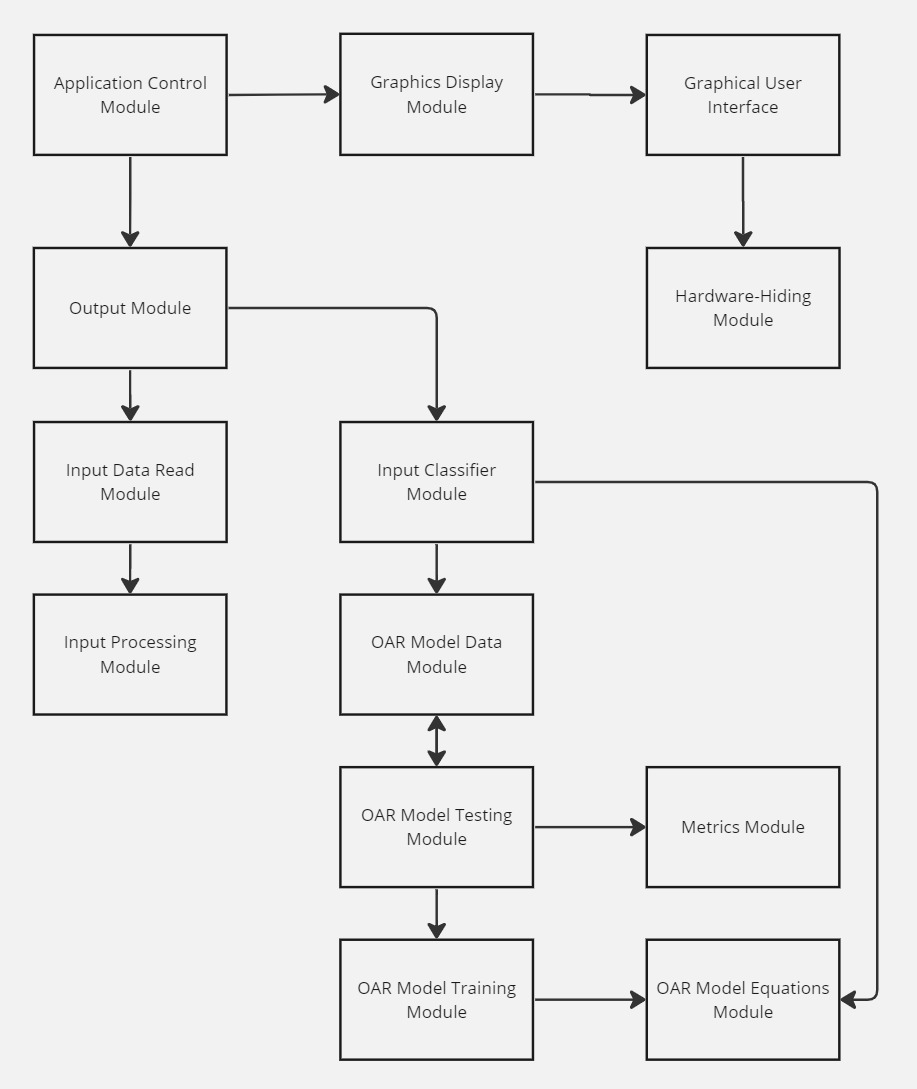
\includegraphics[width=0.7\textwidth]{OAR_UH}
\caption{Use hierarchy among modules}
\label{FigUH}
\end{figure}

\bibliographystyle {plainnat}
\bibliography{../../../refs/References}

\newpage{}

\end{document}